\section{\texorpdfstring{Vyjádření znaménka - záporná čísla}{Vyjadreni znamenka - zaporna cisla}}

% =====================================================================================================================
	\begin{frame}
    \frametitle{Zobrazení záporných čísel}
		\boldmath
    
    \begin{itemize}
      \item Polyadické soustavy obsahují pouze nezáporná čísla.
      \item Hledáme transformaci mezi omezenou množinou celých čísel a omezenou množinou čísel nezáporných.
      \item Očekáváme binární reprezentaci pro HW aplikace - zápis do registru v mikroprocesoru.
      \item Očekáváme snadný algoritmus provádění aritmetických operací - ALU v mikroprocesoru.
      \item Nejpoužívanější číselné kódy
      
      \begin{itemize}
        \item přímý,
        \item aditivní,
        \item doplňkový.
      \end{itemize}
      
    \end{itemize}
    
	\end{frame}
  
% =====================================================================================================================
	\begin{frame}
    \frametitle{Přímý kód}

		\begin{minipage}{0.49\textwidth}
      \small
      \begin{itemize}
        \item Volba znaménka dle MSB \\
              + odpovídá 0 \\
              - odpovídá 1
        \item Zbývající bity reprezentují absolutní hodnotu
        \item Reprezentace je přirozená člověku
        \item Nepraktické rozšiřování na více bitů
      \end{itemize}
      
		\end{minipage}
		\begin{minipage}{0.49\textwidth}
      \boldmath
      \begin{center}
        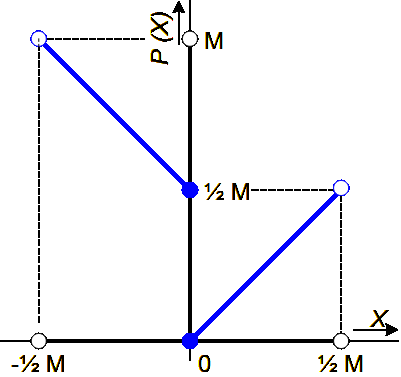
\includegraphics[width=\textwidth]{fig/primy_kod.png}
      \end{center}
      \small
      \[
      P(X) =
        \begin{Bmatrix*}[l]
          X & pro\: X > 0\\
          \left| X \right| + \frac{1}{2}M & pro\: X\leq 0
        \end{Bmatrix*}
      \]
      
		\end{minipage}
		
	\end{frame}
  
% =====================================================================================================================
	\begin{frame}
    \frametitle{Aditivní kód}

		\begin{minipage}{0.49\textwidth}
      \small
      \boldmath
      \begin{itemize}
        \item Kód s posunutou nulou o $K$
        \item Zachovává relace $>,<,=$
        \item Jednoduchý převod
        \item Speciálně pro $K= M/2$ lze negací MSB získat totéž číslo v doplňkovém kódu
        \item Obtížné rozšiřování na více bitů
      \end{itemize}
      
		\end{minipage}
		\begin{minipage}{0.49\textwidth}
      \boldmath
      \begin{center}
        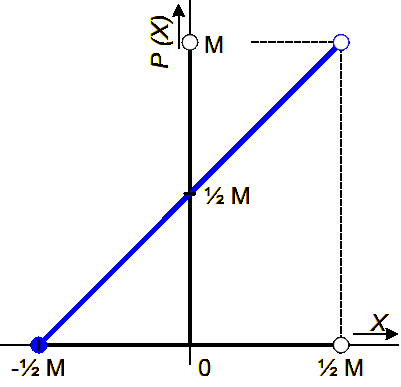
\includegraphics[width=\textwidth]{fig/aditivni_kod.png}
      \end{center}
      \small
      \[
        \begin{matrix*}[l]
          P(X) = X + K \\
          X \geq -K,\: X \leq M - K
        \end{matrix*}
      \]
      
		\end{minipage}
		
	\end{frame}

% =====================================================================================================================
	\begin{frame}
    \frametitle{Doplňkový kód - 1. doplněk}

		\begin{minipage}{0.49\textwidth}
      \small
      \boldmath
      \begin{itemize}
        \item Doplněk do modulu mřížky $M$
        \item Problém s přítomností dvou nul při přetečení
        \item Snadný převod mezi kladnou a zápornou hodnotou:
      \end{itemize}
      
      \tiny
      \begin{center}
        \begin{tabular}{|c|c||c|c|}
        \hline
        $(X)_{10}$ & $(X)_{2}$ & $(-X)_{10}$ & $(-X)_{2}$ \\
        \hline
        0 & 000 & -0 & 111 \\
        1 & 001 & -1 & 110 \\
        2 & 010 & -2 & 101 \\
        3 & 011 & -3 & 100 \\
        \hline
        \end{tabular}
      \end{center}
      \small
      Jen inverze všech bitů.
      
		\end{minipage}
		\begin{minipage}{0.49\textwidth}
      \boldmath
      \begin{center}
        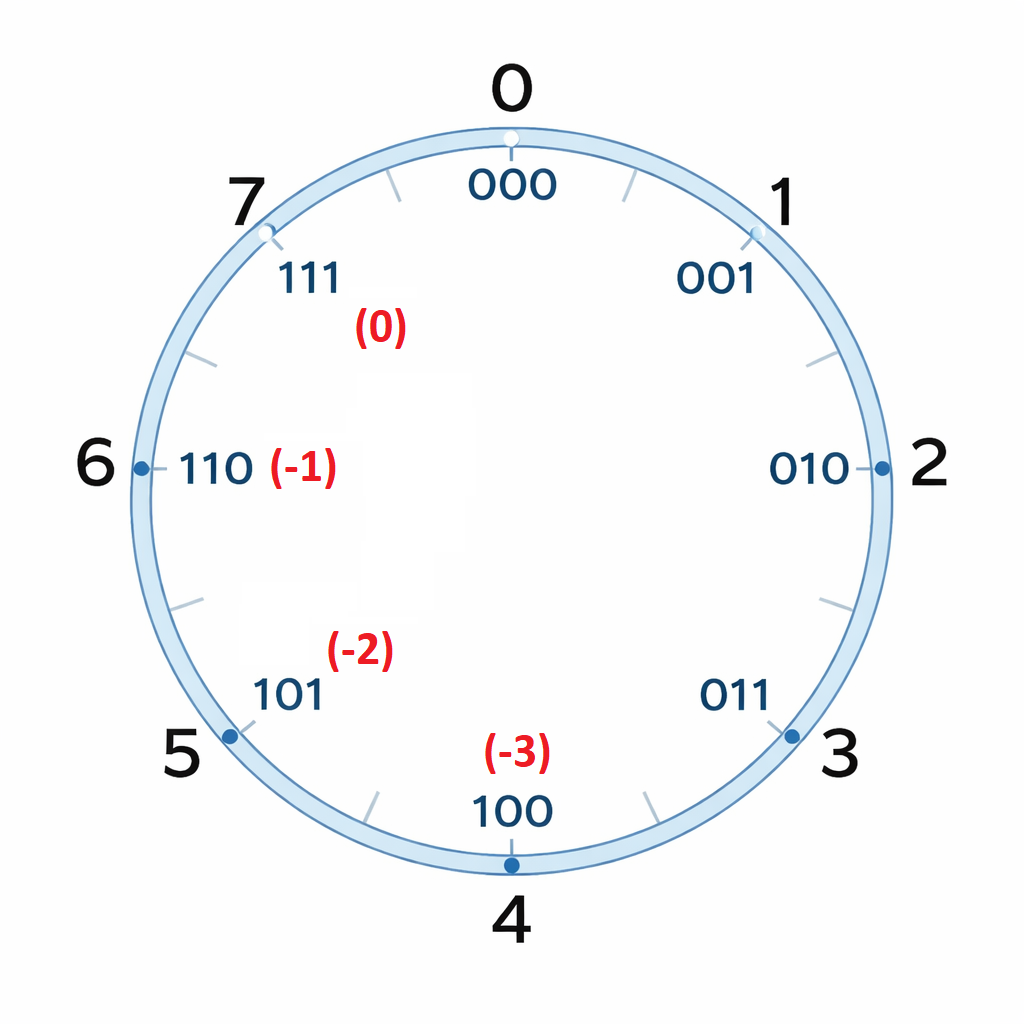
\includegraphics[width=\textwidth]{fig/cifernik_1st_doplnek.png}
      \end{center}
     
		\end{minipage}
		
	\end{frame}
  
% =====================================================================================================================
	\begin{frame}
    \frametitle{Doplňkový kód - 1. doplněk - výpočty}

		\begin{minipage}{0.49\textwidth}
      \small
      \boldmath
      $1 + 2 = [1] + [2] = [3] = 3$ \textcolor{teal}{\textbf{OK}}
      $1 - 2 = [1] + [5] = [6] = -1$ \textcolor{teal}{\textbf{OK}}
      $-1 + 2 = [6] + [2] = [8] = 0$ \textcolor{red}{\textbf{X}}
      $-1 - 2 = [6] + [5] = [11] = 3$ \textcolor{red}{\textbf{X}}
      
      \vspace{4mm}
      \textbf{Problém s přetékáním:}
      
      
		\end{minipage}
		\begin{minipage}{0.49\textwidth}
      \boldmath
      \begin{center}
        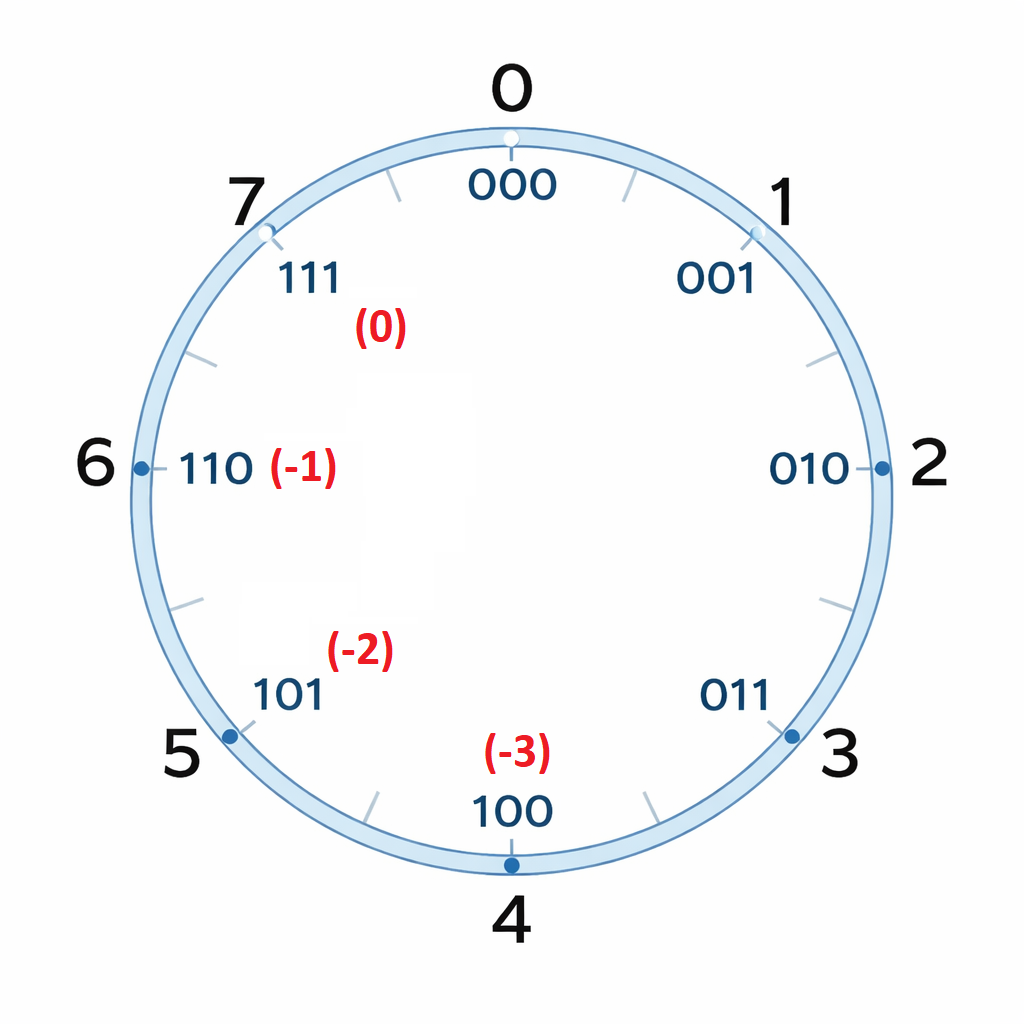
\includegraphics[width=\textwidth]{fig/cifernik_1st_doplnek.png}
      \end{center}
     
		\end{minipage}
		
	\end{frame}
  
% =====================================================================================================================
	\begin{frame}
    \frametitle{Doplňkový kód - 2. doplněk}

		\begin{minipage}{0.49\textwidth}
      \small
      \boldmath
      \begin{itemize}
        \item Doplněk do maxima mřížky $M-1$
        \item Jen jedna nula
        \item Relativně snadný převod mezi kladnou a zápornou hodnotou:
      \end{itemize}
      
      \tiny
      \begin{center}
        \begin{tabular}{|c|c||c|c|}
        \hline
        $(X)_{10}$ & $(X)_{2}$ & $(-X)_{10}$ & $(-X)_{2}$ \\
        \hline
        0 & 000 & -0 & / \\
        1 & 001 & -1 & 111 \\
        2 & 010 & -2 & 110 \\
        3 & 011 & -3 & 101 \\
        4 & / & -4 & 100 \\
        \hline
        \end{tabular}
      \end{center}
      \small
      Inverze všech bitů + 1.
      
		\end{minipage}
		\begin{minipage}{0.49\textwidth}
      \boldmath
      \begin{center}
        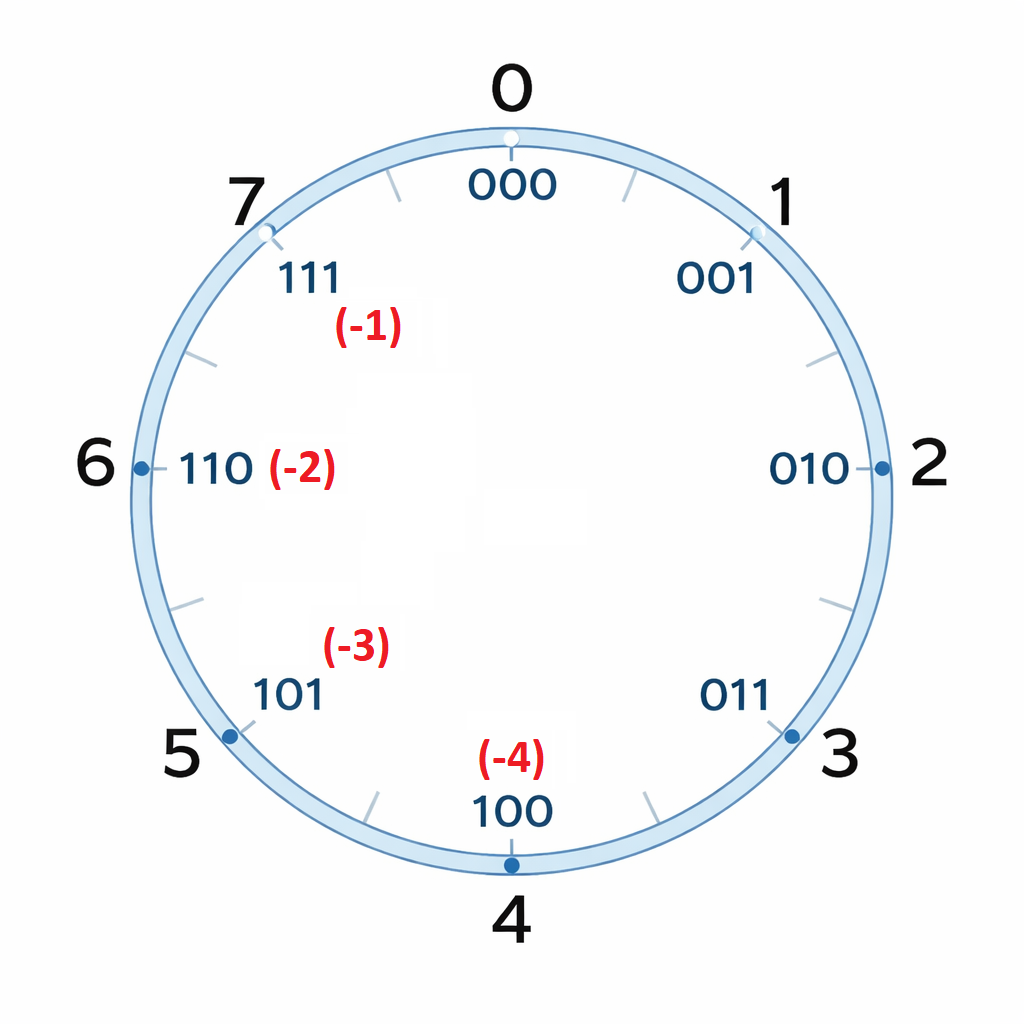
\includegraphics[width=\textwidth]{fig/cifernik_2nd_doplnek.png}
      \end{center}
     
		\end{minipage}
		
	\end{frame}
% =====================================================================================================================
	\begin{frame}
    \frametitle{Doplňkový kód}

		\begin{minipage}{0.49\textwidth}
      \small
      \boldmath
      \begin{itemize}
        \item Znaménko je patrné z MSB
        \item Snadná HW implementace a výpočty
        \item Snadné rozšiřování počtu bitů 
        
        \begin{itemize}
          \item $X\geq 0$ rozšiřuje 0 vlevo 
          \item $X < 0$ rozšiřuje 1 vlevo 
        \end{itemize}
        
      \end{itemize}
      
		\end{minipage}
		\begin{minipage}{0.49\textwidth}
      \boldmath
      \begin{center}
        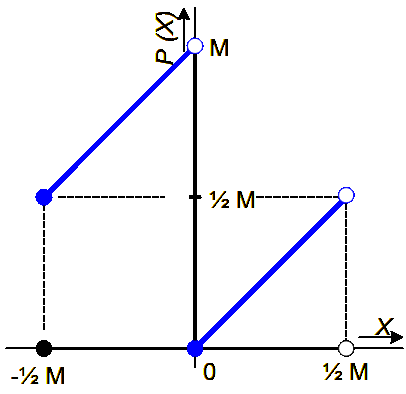
\includegraphics[width=\textwidth]{fig/doplnkovy_kod.png}
      \end{center}
      \small
      \[
      P(X) =
        \begin{Bmatrix*}[l]
          X & pro\:X \geq 0\\
          X + M & pro\:X < 0
        \end{Bmatrix*}
      \]
      
		\end{minipage}
		
	\end{frame}